% ------------ NEW CHAPTER ------------
\chapter{Návrh riešenia}
Kapitola bude zahŕnať použitý software pre tvorbu klasifikátorov a neurónových sieti, špecifikáciu hardwaru na ktorom bude trénovanie priebiehať.
Ďalej priblíži zbroje a spôsoby pre získanie, spracovanie a rozdelenie dát zbraní určených pre klasifikáciu typu a určenie náklonu v scéne.
Následne opíše celkový navrhovaný postup, od predspracovania obrazu až po zber výsledkov a určenie presnosti daných klasifikátorov.
Celá kapitola bude vychádzať z informácií ktoré boli spomenuté v kapitole \ref{chap:technologie}.



\section{Použitý software a hardware}
\label{sec:softwarehardware}
Prvým bodom pri návrhu riešenia je dôležité vybrať správny programovací jazyk a nástroje, ktoré sú pre riešenie daného problému vhodné
    a ktoré môžu uľahčiť aj celkovú implementáciu.

V kapitole \ref{sec:frameworks} bol vytvorený základny prehľad populárnych nástrojov pre tvorbu klasifikátorov, neurónových sietí a predspracovanie obrazu.
Vzhľadom na porovnanie týchto nástrojov, bude pre túto prácu použitý programovací jazyk Python, knižnica Keras pre tvorbu konvolučných neurónových sietí, ktorá
    ako svoj backend bude využívať knižnicu TensorFlow.
A následne pre klasický prístup ku klasifikácií obrázkov bude použitá knižnica Scikit-learn a Scikit-image pre implementáciu predspracovania obrazu.

Keďže trénovanie klasifikátorov a neurónových sietí je výpočetne náročna operácia, je vhodné použiť výkonný hardware a akceleráciu výpočtou na GPU.
Pre túto prácu bude použitý počitač so štvorjadrovím procesorom i7-6700HQ, veľkosťou operačnej pamäte 16 GB a grafickou kartou Nvidia GeForce 940MX.
Na použitom počitači bude nainštalovaný 64-bitový operačný systém Fedora 27.



\section{Trénovacia databáza zbraní}
- Z kade navrhujem cerpat data pre zbrane, IMDB pre zbrane a ImageNet.
- Dalej od Tomasa nastroj chcem pouzit, ako sa tam generuju data, dat do navrhu screen-shot z toho.

\subsection{Generovanie dát z 3D modelov}
- Pouzitie tomasovho softwaru
- Program pre konvertovanie modelov do spravneho formatu

\subsection{Augmentácia obrázkov}
- Opisat argumenty datagen v Keras ktore chcem pouzivat.



\section{Klasifikácia typu zbrane}
Jedným z cieľou tejto práce je klasifikovať typy zbraní do 2 kategórií, a to na krátke a dlhé zbrane.
Táto klasifikácia môže prebiehať niekoľkými spôsobmi, prehľad týchto prístupov bol zhrnutý v kapitolách \ref{sec:detekcia} a \ref{sec:klasifikacia}.
Pre klasifikáciu v tejto práci bude použitých niekoľko z týchto prístupov a vo výsledku budú porovnané, ktorý dosiahol najlepšie výsledky.

Prvé riešenie bude spočívať v klasickom prístupe, ktoré pozostáva z predspracovania vstupných dát pomocou prekonvertovania dát do šedotónoveho obrazu a histogramu orientovaných prechodov (vid. \ref{sec:preprocessing}).
Na tieto predspracované dáta bude v jednom z riešení použitý K-Nearest-Neighbor klasfikátor, pre druhé riešenie bude použitý SVM klasifikátor, testovanie
    a porovnávanie výsledkov môže prebiehať s rôznymi konfiguráciami týchto klasifikátorov.
\begin{enumerate}
    \item[$\bullet$] Pre \textbf{K-Nearest-Neighbor}, knižnica scikit-learn poskytuje 2 rôzne implementácie tohto klasifikátora.
    Trieda \textit{KNeighborsClassifier} klasifikuje na základe $k$ najbližšich susedov, kde $k$ je celé číslo špecifikované užívateľom.
    
    Druhá implementácia je trieda \textit{RadiusNeighborsClassifier} ktorá klasifikuje na základe počtu susedov v rámci pevného polomeru $r$ každého trénovacieho bodu,
        kde $r$ je hodnota s pohyblivou desatinou čiarkou určená užívateľom\footnote{\url{http://scikit-learn.org/stable/modules/neighbors.html\#nearest-neighbors-classification}}.
    \item[$\bullet$] Pre \textbf{Support Vector Machines}, scikit-learn obsahuje 3 triedy \textit{SVC}, \textit{NuSVC} a \textit{LinearSVC} pre viac-triednu
        klasifikáciu s možnosťou použitia rôznych typov jadier \footnote{\url{http://scikit-learn.org/stable/modules/svm.html\#custom-kernels}}.
    %\item[$\bullet$] \textbf{Multi Layer Perceptron}
\end{enumerate}

Pre dalšie riešenie klasfikácie zbraní budú použité dve konvolučné neurónové siete, ktorých výsledky budú porovnané, podrobná architektúra sieti je opísana v kapitole \ref{sec:architekuraCNN}.
Predspracovanie vstupných dát bude pozostávať z normalizacie hôdnot RGB zložiek pixelov, nastavenia rovnomernej veľkosti strán obrázka (vid. \ref{sec:preprocessing})
    a následnej augmentácií dát pre zväčsenie počtu vstupných dát (vid. \ref{subsec:augmentacia}).



\section{Určenie náklonu zbrane}
Druhý z cieľou tejto práce je určenie náklonu zbrane v obraze.
Tento náklon bude určeny v 3 osách.
Dôležité je spomenúť že názvy ós sú pomenované podľa tých ktoré sa používajú v letectve, vid. obrázok \ref{pic:airplaneaxis}.
\begin{figure}[H]
    \centering
    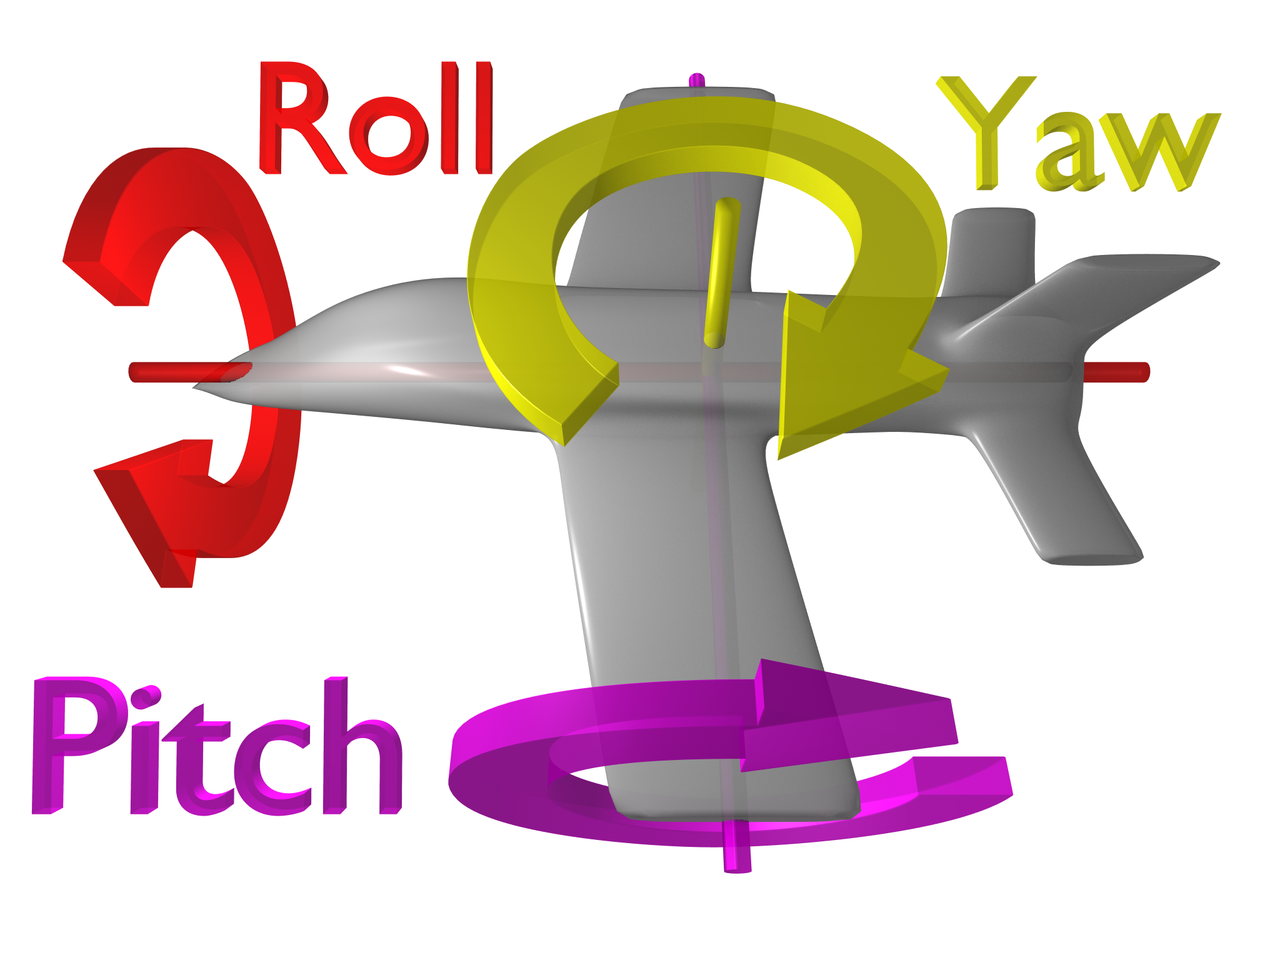
\includegraphics[width=0.5\textwidth]{airplane-axis}
    \caption{Mená ós pre letectvo.}
    \label{pic:airplaneaxis}
\end{figure}

Tento problém je môžné preniesť do klasifikácie, preto pre riešenie tohto problému budú použité konvolučné neurónové siete, ktorých všeobecná architektúra je popísana v \ref{sec:architekuraCNN}.
Výsledok poslednej vrtsvy softmax klasfikátora bude 72 výstupov ktoré budú určovať o aký uhol je zbraň natočená.
Každá zo 72 kategórií bude zastupovať rozpätie 5 stupňov, ciže celkovo sa určí náklon zbrane v celom rozsahu od 0 do 360 stupňov.

Postup predspracovania obrazu bude rovnaký ako pri klasfikácií zbraní pomocou konvolučných neurónových sieti, normalizácia, úprava rozmeru vstupu na štvorec a augmentácia dát (vid. \ref{subsec:augmentacia})
Pre každú os bude natrénovaná samostatná konvolučná neurónová sieť, výsledok bude teda obsahovať 3 natrénované modely.


\subsection{Odchylka chyby}
Kedže knižnica nemá priamu podporu pre určenie


\section{Zhrnutie kapitoly}



\begin{comment}

    \section{Klasifikácia typu a určenie náklonu zbrane}
    Prvým bodom pri návrhu riešenia je výber programovacie jazyka a nástrojov, ktoré sú prispôsobné pre riešenie daného problému a tak uľahčujú výslednú implementáciu.
    Pre riešenie tejto práce bol vybraný programovací jazyk Python spolu s nástrojmi ktoré boli spomenúte už vyššie vid. sekcia \ref{sec:TensorflowKeras} a \ref{sec:scikitlearn}.
    Výsledny program bude mať za úlohu klasifikovať typ zbrane (krátka, dlhá) zo vstupného obrázku a následne určiť jej náklon.
    Pre klasifikáciu zbrane do daných kategórií sa ponúka niekoľko postupov klasifikácie, ktoré sú podrobne opísane v sekcíí \ref{sec:klasifikacia},
        pri určovaní náklonu zbrane v obraze môžeme použiť konvolučné neurónové siete.

\end{comment}

\begin{comment}

    \subsection{implementacia a vysledky- poznamky}
    \begin{enumerate}
        \item[$\bullet$] Z kade som realne cerpal data nakoniec
        \item[$\bullet$] Ako prebiehala augmentacia dat, opisat funkcie ktore sa pouzivaju pre dogenerovanie obrazkov a nazov tried ktore to implementuju.
        \item[$\bullet$] Obrazok trenovanie neuronovej siete
        \item[$\bullet$] Dosiahnute vysledky
        \item[$\bullet$] vytvorit velku prehladnu tabulku pre budu kompletne vysledky, tak ako to je na git-e opisane
    \end{enumerate}

\end{comment}

